\section{Efficiency}\label{subs:efficiency}
In \cref{subs:recipequeue} we illustrate how we make search for the fastest timed trace more efficient, by ordering how recipes are placed onto a factory. By applying such order we are trying to keep down the global state space like how the bourgeois tries to keep down the proletariat.   

This is not the only part of the model, in which we have tried to make our search more efficient. We have strayed from going deeper into it until now, as it does not impact the overall functionality of the model. Yet it does greatly impact runtime. 

The use of urgent channels and committed locations are what mainly speeds up the search.

Committed locations ensure that globally no action may be taken and no time may pass before leaving a location. This ensures that some processes stay atomic, such as the handshake and work on recipes described in \cref{subs:recipe}. This guards us from the interference of other instance, but also greatly reduces the search space.

Urgency is an attribute that can be applied to different channels. Having a channel be urgent means that no time may pass, if we are in a state, where we can synchronize on the channel. In \emph{ModuleWorker} on \cref{subs:moduleworker} the intern channel is urgent. This means that when the guards evaluate to true, then we will synchronize on \emph{intern} as soon as possible. Not allowing the system the possibility of waiting again reduces the state space. There are transitions we wish to make urgent, such as from \emph{Done} to \emph{Working}, where they are not already communicating on a channel. We solve this by creating a new simple template called \emph{Urgent}. An instance of this will continuously try to synchronize on the urgent \emph{urg} channel. Thus we can add a synchronization on this channel to any non-urgent transition to make it urgent. 

A big difficulty with working with committed locations and urgent channels is that we sometimes need to be able to wait. This is the case when passing from \emph{ModuleWorker} to \emph{ModuleTransporter} through the intern channel as mentioned above. We can not safely make \emph{intern} urgent, if we may synchronize on it from \emph{ModuleWorker} but not   \emph{ModuleTransporter}. This will lead to unwanted deadlock.  Therefore, the guard on this particular transition states that it must only be taken, if the \emph{ModuleTransporter} is in idle and can communicate. We use this technique throughout the model, applying guards so that we may safely make our channels urgent. 

In order to shave more off the state space, we have also created priorities between channels using built-in UPPAAL priority feature. This can be seen in \cref{code:cp}. By placing this order we do not allow the model checker to synchronize on a certain channel if a channel of a higher priority may be synchronized on. This helps guide us when there is an ambiguous choice of which channel to communicate on.

There is however not a strong or weak timed bisimilar equivalence between any processes of the system without priorities and the system with. Obviously, because there will be instances, where the unprioritized system will be able to perform a transition, where the prioritized system will not. However, our model is designed in such a way that when an instance can communicate on a channel, it will not change its local state until allowed to communicate. This entails that it does not leave the location from which it tries to communicate. Two processes wanting to communicate will as such wait in the same local state until the priorities are in their favour. Thus we ensures that there is some grander execution equivalence between the prioritized system and the unprioritized system. The only difference is that we have to deal with a smaller state space when using priorities. \todo{Bedre forklaring}
\todo{Har kaldt processor for instanser her igennem}

An issue is that even with channel priorities, we may have two transitions communicating on the same channel type, which again leaves us with an ambiguous order of execution. To get around this we also prioritize system instances. If we ever get into this situation, we pick the transition involving instances of the highest priorities. 

\lstinputlisting[language=C, caption=Channel priorities, captionpos = b, label={code:cp}, float]{codeRelated/UPPAAL/channelpriorities.txt}


A feature which UPPAAL templates lack is a user-defined constructor, which would allow us to execute code right when an instance is made. We need this feature in templates such as \emph{ModuleQueue} in \cref{subs:modulequeue}, where we need to set up the array, which implements the queue. To get around this, we add an initial location to the template. To transition from this location, the instantiating functions have to be called. The issue here is that with N instances having to be instantiated, there are N! sequences of performing instantiation. Again, this greatly increases our state space. To get around this, we use a queueing system similar to \emph{RecipeQueue} in \cref{subs:recipequeue}. This is implemented with the \emph{Initializer} template as seen in \cref{fig:initializer}. Each instance, which needs to have code run upon instantiation, is given an instantiation id. When instantiating the \emph{Initializer}, we give it an array, which orders all these ids. The \emph{Initializer} then starts to instantiate the instances in the order given to it by synchronizing on the \emph{initialize} channel. As the \emph{Initializer}'s main location is committed, nothing may occur until all needed instances have been synchronized with. Once all instantiation has been done, the \emph{Intanializer} is forced to move into a dead state and we need not to worry about it anymore.    

\begin{figure}[h]
\centering
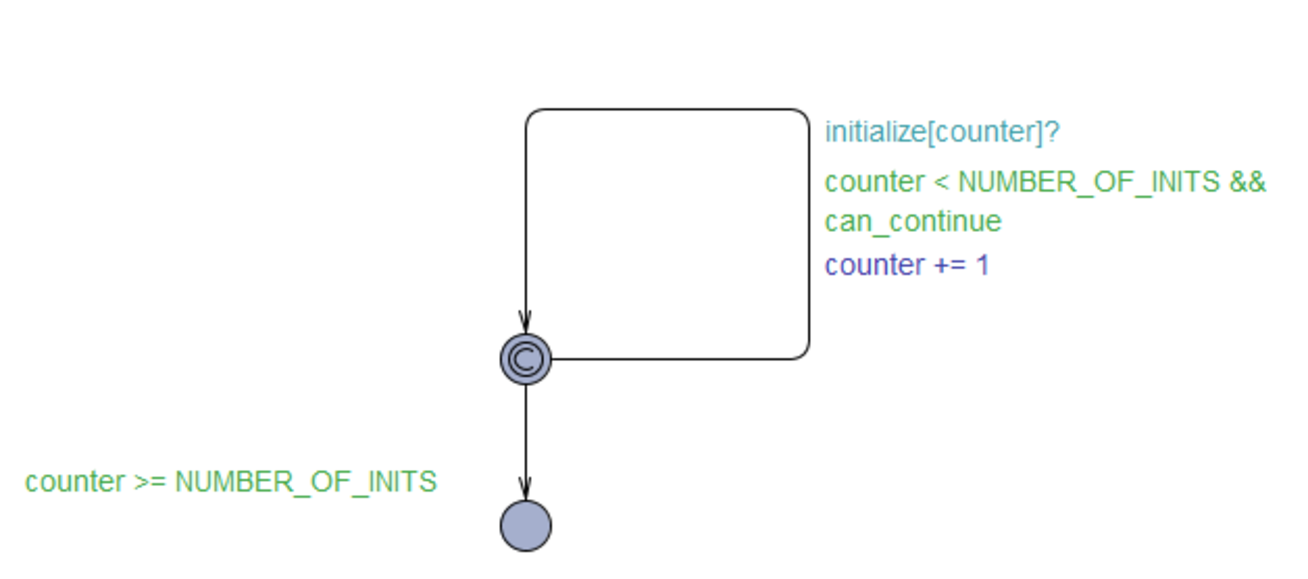
\includegraphics[width=\textwidth]{init.pdf}
\caption{The Initialzier template}
\label{fig:initializer}
\end{figure}

